
\section{Low Speed Wind Tunnel}

The Old Dominion University low 
speed wind tunnel (LSWT) was outfitted with a bi-wing axial vortex generator. 
The tunnel has a large test section measuring 2.134$m$ wide by 2.438$m$ 
tall and a small test section measuring 1.219$m$ wide by 0.911$m$ tall. The 
wind tunnel air is propelled with a frequency controlled 125 Horsepower motor. 
Flow velocity was manipulated directly by manually controlling
voltage supplied to the controller. 
The small test section has a total length of 2.438$m$, and the vortex generator 
spaned the 0.911$m$ height of the test section and was 
mounted 0.610$m$ from the front end, leaving 1.829$m$ downstream for the axial 
vortex to develop. The 3x4 foot test section has a functional free stream 
velocity range between 12 and 55 meters per second or between 35 and 120 miles 
per hour.

\begin{figure}[H]
\centering
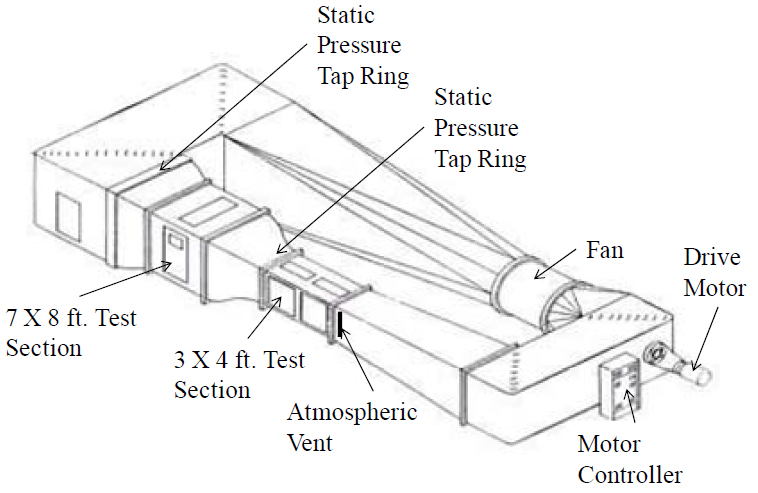
\includegraphics[width=5in]{figs/setup/odulswt_diagram}
\caption{ODU Low speed wind tunnel.}
\label{fig:odulswt}
\end{figure}

The entire interior of the test section remained vacant and unobstructed with 
the exception of the vortex generator. 
No internal traverse systems or structures 
were present during PIV data acquisition unless otherwise indicated. Tunnel 
velocity was determined by direct measurement of dynamic pressure ($q$), which 
is monitored and controlled by the tunnel control PC. Figure 
\ref{fig:control_diagram} contains a schematic diagram of the systems under the 
wind tunnel control PC.

\begin{figure}[H]
\centering
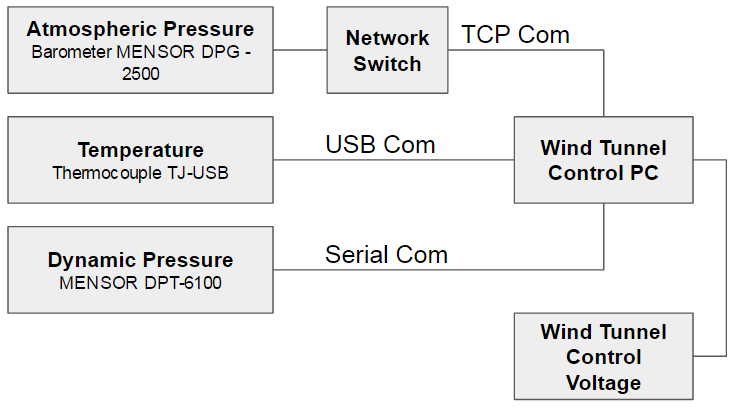
\includegraphics[width=5in]{figs/setup/odulswt_control}
\caption{Schematic diagram of systems under wind tunnel PC control.}
\label{fig:control_diagram}
\end{figure}


